\section{Learning-based Whole-Body Controller}
The model-based planner predicts the desired racket striking position $\hat{\mathbf{p}}_{\mathrm{racket}}$, velocity $\hat{\mathbf{v}}_{\mathrm{racket}}$, and timing $t_{\mathrm{strike}}$. 
These predictions are provided to the learning-based Whole Body Controller (WBC), which generates the corresponding whole-body motions for the humanoid. We train the WBC policy $\pi_\text{WBC}$ in Isaac Lab~\cite{mittal2023orbit} and deploy it to the real robot in a zero-shot manner. The policy is trained end-to-end using the model-free reinforcement learning algorithm PPO~\cite{schulman2017proximal}. The joint PD gains are set heuristically following~\cite{liao2025beyond}.

\begin{table}
\centering
\caption{Observation spaces for the policy (actor) and critic. The critic receives additional privileged information during training.}
\begin{tabular}{lcc}
\toprule
\textbf{Observation} & \textbf{Actor} & \textbf{Critic} \\
\midrule
Base angular velocity ($\bm{\omega}_{\mathrm{base}}\in\mathbb{R}^3$) & \checkmark & \checkmark \\
Projected gravity vector ($\mathbf{g}_{\mathrm{base}}\in\mathbb{R}^3$) & \checkmark & \checkmark \\
Base forward vector ($\mathbf{e}_{\mathrm{base},x}\in\mathbb{R}^2$) & \checkmark & \checkmark \\
Target base position ($\hat{\mathbf{p}}_{\mathrm{base},xy}-\mathbf{p}_{\mathrm{base},xy}\in\mathbb{R}^2$) & \checkmark & \checkmark \\
Target racket position ($\hat{\mathbf{p}}_{\mathrm{racket}}\in\mathbb{R}^3$) & \checkmark & \checkmark \\
Target racket velocity ($\hat{\mathbf{v}}_{\mathrm{racket}}\in\mathbb{R}^3$) & \checkmark & \checkmark \\
Time to strike ($t_{\mathrm{strike}}\in\mathbb{R}$) & \checkmark & \checkmark \\
Joint positions ($\mathbf{q}\in\mathbb{R}^{29}$) & \checkmark & \checkmark \\
Joint velocities ($\dot{\mathbf{q}}\in\mathbb{R}^{29}$)& \checkmark & \checkmark \\
Previous action ($\mathbf{a}_{\mathrm{last}}\in\mathbb{R}^{29}$)& \checkmark & \checkmark \\
Base linear velocity ($\mathbf{v}_{\mathrm{base}}\in\mathbb{R}^3$) & -- & \checkmark \\
Bodies' pose ($\mathbf{T}_\mathcal{B}\in\mathbb{R}^{7|\mathcal{B}|}$) & -- & \checkmark \\
Time left in current episode ($t_{\mathrm{left}}\in\mathbb{R}$) & -- & \checkmark \\
\makecell[l]{Reference joint positions and velocities \\ ($[\hat{\mathbf{q}}, \hat{\dot{\mathbf{q}}}]\in\mathbb{R}^{58}$)} & -- & \checkmark \\
\bottomrule
\end{tabular}
\label{tab:obs_spaces}
\end{table}

\subsection{Human Motion References}
\label{subsec:hmr}

We extend the idea of generating \textit{instantaneous} racket motion close to a ``comfort posture" in \cite{mulling2010biomimetic, mulling2011biomimetic} to generating \textit{continuous} humanoid motion close to two swinging references: \textbf{forehand} and \textbf{backhand}. Note that while \cite{mulling2013generalizestrike} synthesizes a mixture of motor primitives controller from kinesthetic teach-ins, we use video-based demonstrations. First, we record a video clip of a human performing the swing. A corresponding SMPL \cite{loper2023smpl} motion clip is reconstructed from the video using GVHMR~\cite{shen2024world}, and then re-targeted to the humanoid robot using GMR~\cite{ze2025gmr, ze2025twist}. The resulting motion clip contains base pose and joint positions at 30\,Hz.

Following the approach of BeyondMimic~\cite{liao2025beyond}, we enhance the motion for better tracking. We first interpolate the base pose and joint positions from 30\,Hz to 50\,Hz, matching the control frequency of the policy. Then, base linear velocities, angular velocities, and joint velocities are computed using central differencing. Using forward kinematics, we obtain the pose $\mathbf{T}_{b}$ and twist $\mathbf{V}_{b}$ for each body $b \in \mathcal{B}$. Since we only track the motion of the upper body, $\mathcal{B}$ contains only the bodies above the pelvis (pelvis, torso, and arms). The pelvis is chosen as the anchor body $b_{\mathrm{anchor}}$, and the desired pose of other bodies is computed as in~\cite{liao2025beyond}. After processing, each motion clip contains 94 frames (1.88\,s) with the striking occurring at the $43^{\mathrm{nd}}$ frame (0.86\,s).

\begin{figure}
    \centering
    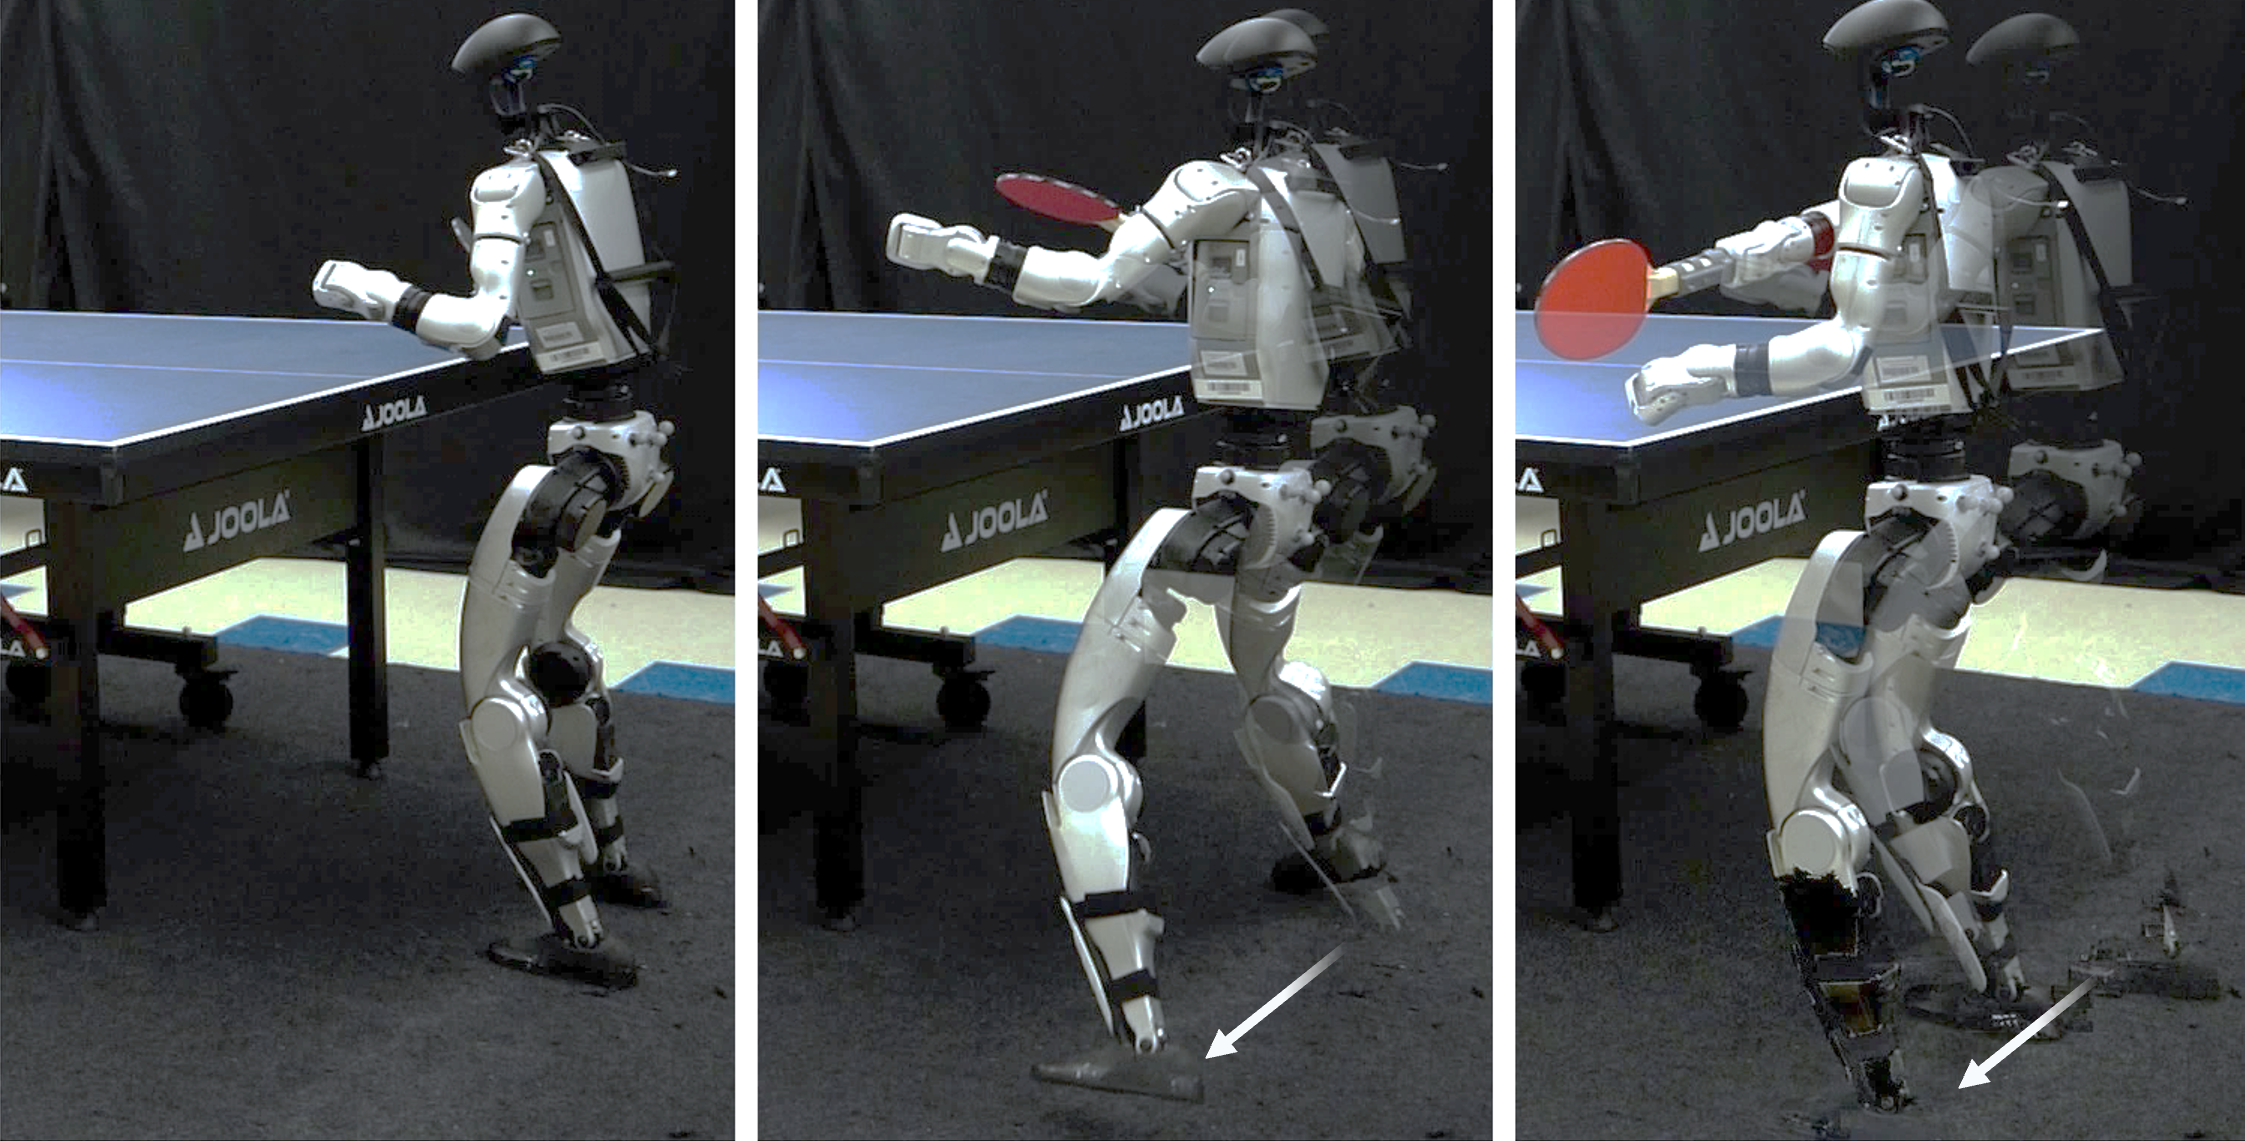
\includegraphics[width=1\linewidth]{figures/side_jump.png}
    \caption{\textbf{Real-world rapid reaching motion.} The whole-body control policy enables agile reaching motions, allowing the robot to swiftly transition from the right side of the table to the left while maintaining balance and successfully striking the ball.}
    \label{fig:side_jump}
\end{figure}

\subsection{Markov Decision Process (MDP) Setting}

\subsubsection{Separate Commands for Base and Racket}
Instead of using the global racket position and velocity at the striking time as commands~\cite{ma2025learning}, we separate the commands for the base and the racket to improve training efficiency. The first command $\hat{\mathbf{p}}_{\mathrm{base},xy}$ specifies the desired base position in the world frame, encouraging the robot to arrive at the target location in time. The second command $[\hat{\mathbf{p}}_{\mathrm{racket}}, \hat{\mathbf{v}}_{\mathrm{racket}}]$ specifies the racket position relative to the base and the racket velocity (both expressed in the world frame). The desired base orientation is always set to face forward.

To enable the policy to perform consecutive strikes and switch between swing types, each episode lasts 10\,s. After completing a swing, we uniformly sample the next swing type (forehand or backhand) and randomly sample the racket target position, racket target velocity, and base target position at the striking time, conditioned on the swing type. The striking plane is fixed at 0.4\,m in front of the robot, so only the $y$ and $z$ coordinates of the racket target position are sampled. The target regions for forehand and backhand are defined to be non-overlapping.

\subsubsection{Reward Functions}
To generate motions that both resemble the reference motions and track the given commands, we follow~\cite{peng2018deepmimic} and define the total reward as:
\begin{equation}
    r = w_i r_i + w_g r_g + w_r r_r,
\end{equation}
where $r_i$ encourages imitation of the upper body reference motion, $r_g$ rewards tracking of the commanded goals, and $r_r$ provides regularization. $w_i$, $w_g$, and $w_r$ are the corresponding reward weights.

Both $r_i$ and $r_r$ are dense rewards that are applied throughout the entire episode.  
In contrast, $r_g$ contains several sparse terms with relatively high weights.  
For instance, the tracking rewards for the racket position, velocity, and orientation are only activated during a short window around the hitting time, while the base position tracking reward is activated only before the strike, enabling the policy to prepare for transitioning to the next target position after hitting.

\begin{figure}
    \centering
    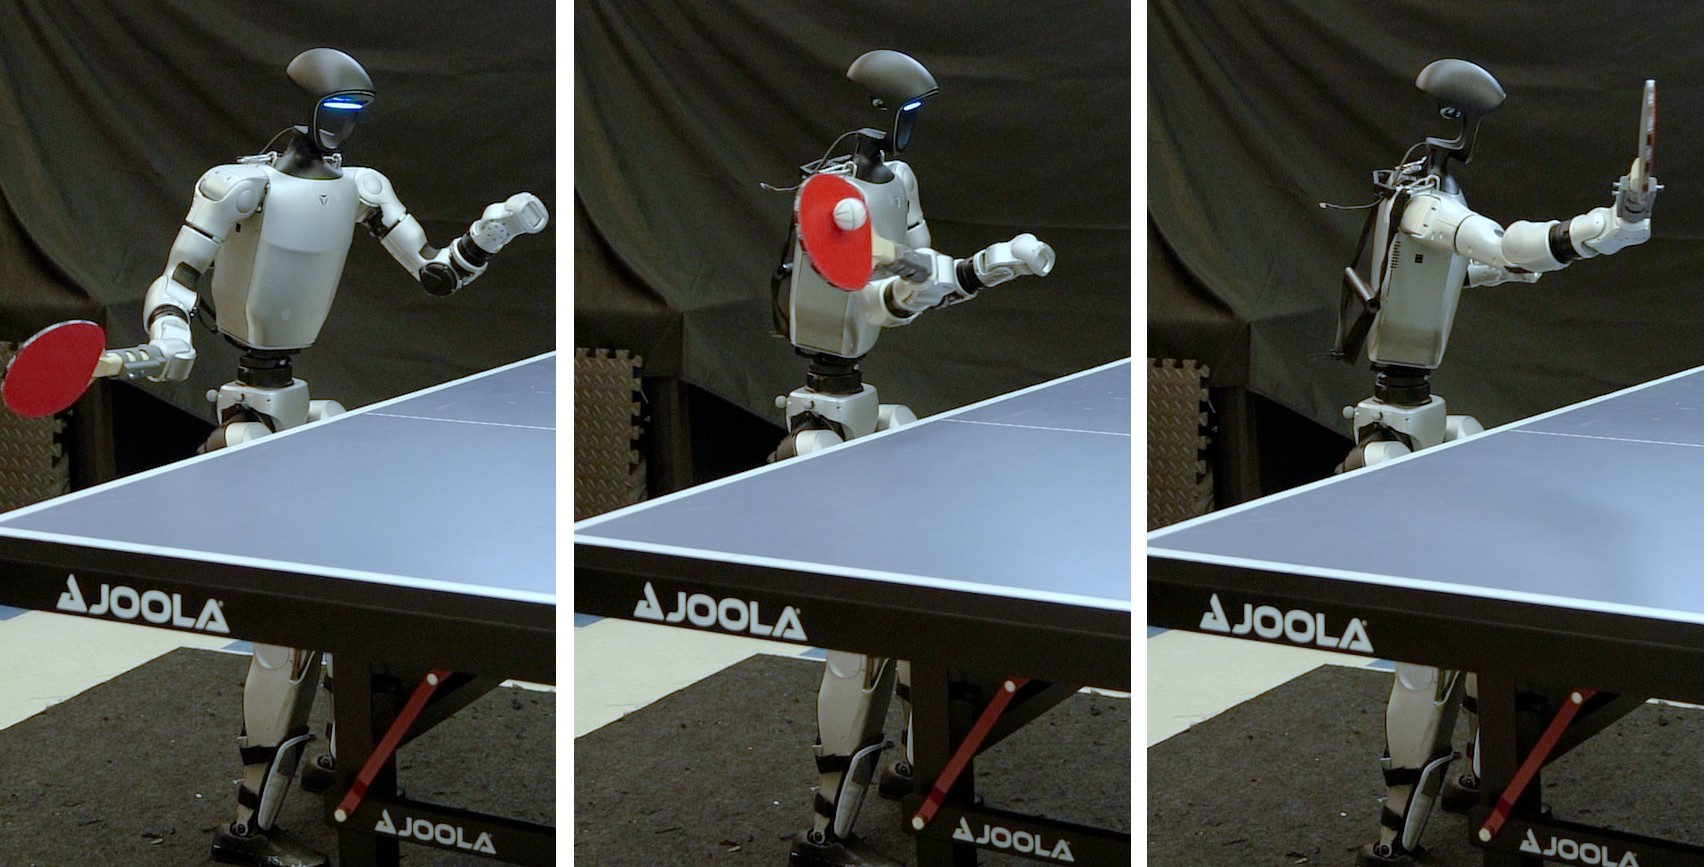
\includegraphics[width=1\linewidth]{figures/hit_motion.jpg}
    \caption{\textbf{Real-world human-like striking motion.} The whole-body control policy generates human-like striking motions, including coordinated waist rotation during hits, which mimics the way humans play table tennis.}
    \label{fig:hit_motion}
\end{figure}


\subsubsection{Asymmetric Actor-Critic}

To provide the critic with additional information unavailable to the policy at deployment, we adopt an asymmetric actor-critic framework for training~\cite{pinto2018asymmetric} (Table~\ref{tab:obs_spaces}).  
For example, to improve reference tracking, we augment the critic’s observations with the robot body poses $T_{\mathcal{B}}$, which facilitate more accurate return estimation. 
Since several terms of $r_g$ are sparse, the episodic return depends on the number of strikes remaining within an episode.  
Therefore, we additionally provide the critic with the time left in the current episode, $t_{\mathrm{left}}$. Both the actor and critic are implemented as multi-layer perceptrons (MLPs) with three hidden layers of sizes 512, 256, and 128.

During deployment, the motion capture system provides the robot base’s position and orientation, which are used to construct $\mathbf{e}_{\mathrm{base},x}$ and $\mathbf{p}_{\mathrm{base},xy}$ in the observation vector. Based on $\mathbf{p}_{\mathrm{base},xy}$ and the predicted racket position $\hat{\mathbf{p}}_{\mathrm{racket}}$, we heuristically determine whether a forehand or backhand strike should be used. This binary variable is then employed to compute the desired base position $\hat{\mathbf{p}}_{\mathrm{base},xy}$. Note that this variable is not included in the policy observations, and it serves only to assist in computing $\hat{\mathbf{p}}_{\mathrm{base},xy}$.
